%
% assembly.tex
%
% Copyright (C) 2020 by SpaceLab.
%
% Flatsat Platform Documentation
%
% This work is licensed under the Creative Commons Attribution-ShareAlike 4.0
% International License. To view a copy of this license,
% visit http://creativecommons.org/licenses/by-sa/4.0/.
%

%
% \brief Board Assembly chapter.
%
% \authors: Gabriel Mariano Marcelino <gabriel.marcelino@spacelab.ufsc.br> and Yan Castro de Azeredo <yan.azeredo@spacelab.ufsc.br>
%
% \institution Universidade Federal de Santa Catarina (UFSC)
%
% \version 0.1.0
%
% \date 2020/24/12
%

\chapter{Board Assembly}

The hardware project has the Bill of Material (BOM) avalaible at its GitHub repository in excel spreeadsheets format. The PCB can be assembled by a Pick-and-place machine using the .txt file found on the hardware/fabrication folder if desired, fiducials labeled FD\# are placed to make this possible.

\section{FlatSat Stabillity Feet}

On the PCB there are labeled MEC1 to MEC12 mouting holes on the edges and in the middle of the board to used for stabillity feet when the board is to be placed on top of a test bench.

\section{DNP Components}

There is only one Do Not Place (DNP) component present in the USB to UART circuit, it is the labeled R4 pad with 0805 size (2012 metric) available for soldering the micro USB type B chassi to GND for Electromagnetic compatibility (EMC) see \ref{fig:R4-pad}. This can be done soldering a zero-ohm resistor for a DC path or capacitor for a high-frequency path between shield and signal ground, see section 2.2.2 of the document \cite{ftdi-usb-hardware-guidelines} for more details.

\begin{figure}[!ht]
    \begin{center}
        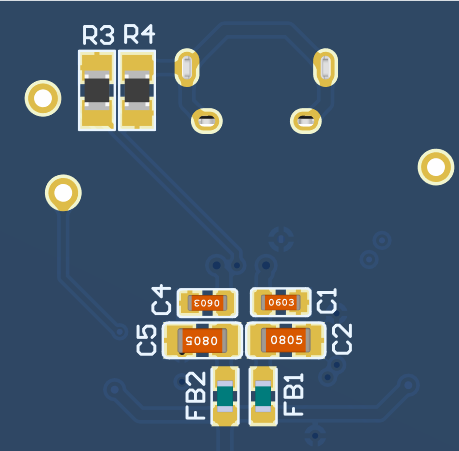
\includegraphics[width=0.5\textwidth]{figures/ft4232h_circuit_bottom.png}
        \caption{Bottom view of the UART to USB converter circuit.}
        \label{fig:R4-pad}
    \end{center}
\end{figure}

\section{Modules Mounting}

The PC104 slots Nº2 to Nº7 are compatible for CubeSat PCB modules that are stacked in middle or the first on top. The slot Nº1 can only be used for the last module on this stack because of the inverted pinout. For the case of the SpaceLab's CubeSat stackup of the core modules, the last module of the stack is the EPS. For this case the EPS needs to be mounted up-side-down on slot Nº1 as can be seen on figure \ref{fig:eps2-mouting}. For other modules any other PC104 slots can be used, the OBDH is showed mouted on figure \ref{fig:obdh2-mouting}. 

\begin{figure}[!ht]
    \begin{center}
        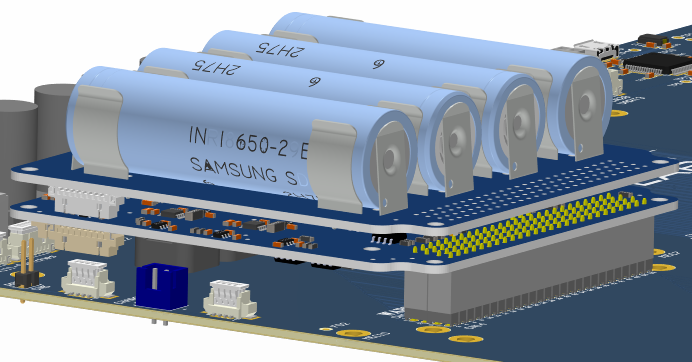
\includegraphics[width=0.8\textwidth]{figures/eps2_mouting.png}
        \caption{EPS mounted on Nº1 slot on a EDA tool.}
        \label{fig:eps2-mouting}
    \end{center}
\end{figure}

\begin{figure}[!ht]
    \begin{center}
        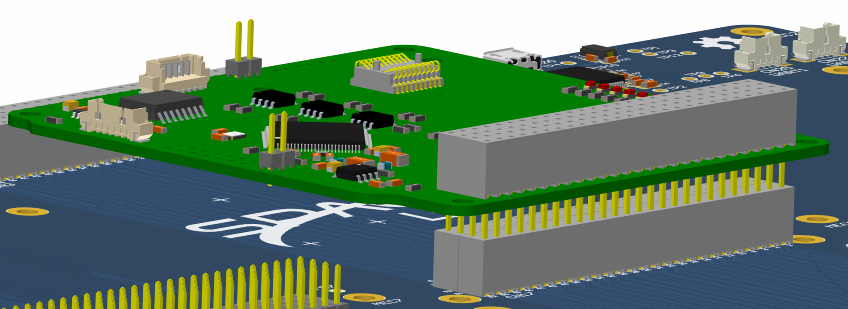
\includegraphics[width=0.8\textwidth]{figures/obdh2_mouting.png}
        \caption{OBDH mounted on Nº2 slot on a EDA tool.}
        \label{fig:obdh2-mouting}
    \end{center}
\end{figure}

\section{Antennas Connection}

Since the SMA connectors present on the board are on the right far side, modules place in the opposite side may not be in reach for the connection. Because of this reason is recommended to use slots Nº1 and Nº4 for non antenna dependents PCBs.